\subsection{Tests}

\paragraph{}
Pour tester notre algorithme nous avons eu besoin de deux choses :
\begin{itemize}
\item une fonction permettant de valider notre solution
\item un fonction permettant de générer aléatoirement des tests
\end{itemize}

\paragraph{}
La méthode \verb?isValid()? qui vérifie la validité de la solution calculée par notre algorithme est donnée par le pseudo-code suivant :
\begin{lstlisting}
isValid(ArrayList<Point> graph, ArrayList<Points> cds, int edgeTreshold) {
	valid = true;
	//build the graph structure of the cds
	ArrayList<NodeVertexDS> graphcds = graph(cds);
	
	//compute connex components
	for( v in graphcds ) {
		for( vn in v.neighbors ) {
			v.disjointsetelement.union(vn.disjointsetelement)
		}
	}
	
	compconnex = new HashSet<DisjointSetElement>();
	for( v in graphcds ) { compconnex.add(v.disjointsetelement.find()); }
	
	if(compconnex.size() > 1) { print("Error on connexity : " + compconnex.size()); valid = false) }
	
	rest = points.clone();
	rest.removeall(cds);
	
	//remove all neighbors of elements of cds from rest
	removeneighbors(rest, cds, edgeTreshold);
	
	if(rest.size() > 0) { print("Error dominating : " + rest.size()); valid = false; }
	
	return valid;
}
\end{lstlisting}

\paragraph{}
Nous avons aussi eu besoin de générer des tests. Pour cela il convient de générer des graphes géométriques de différentes tailles et avec des seuils différents (valeur maximale pour que 2 points soient considérés voisins l'un de l'autre).
Voici le pseudo code du générateur :
\begin{lstlisting}
generateGraph(width, heigth, nb, edgeTreshold) :
	result : ArrayList<Point>;
	while result.size() != nb :
		add random points in result until result.size() == nb
		compute connected components of result
		if there is multiple connected components :
			keep only the biggest connected components in points (remove the points that are in smaller components)
\end{lstlisting}

\paragraph{}
Nous avons ensuite établi plusieurs bases de test :

\begin{figure}[ht]
\begin{center}
\begin{tabular}{|*{3}{c|}}
    \hline
     Nombre de points  & Largeur $\times$ Hauteur  & Seuil \\
    \hline
    100  & 1000 $\times$ 1000 & 50 \\
    \hline
    500  & 1000 $\times$ 1000  & 50 \\
    \hline
    1000  & 1000 $\times$ 1000  & 50 \\
    \hline
    5000  & 1000 $\times$ 1000  & 50 \\
    \hline
    10000  & 1000 $\times$ 1000  & 50 \\
    \hline
\end{tabular}
\end{center}
\captionof{table}{Base de test 1}
\end{figure}

\begin{figure}[ht]
\begin{center}
\begin{tabular}{|*{3}{c|}}
    \hline
     Nombre de points  & Largeur $\times$ Hauteur  & Seuil \\
    \hline
    100  & 1000 $\times$ 1000 & 5 \\
    \hline
    500  & 500 $\times$ 500  & 25 \\
    \hline
    1000  & 1000 $\times$ 1000  & 50 \\
    \hline
    5000  & 5000 $\times$ 5000  & 250 \\
    \hline
    10000  & 10000 $\times$ 10000  & 500 \\
    \hline
\end{tabular}
\end{center}
\captionof{table}{Base de test 2}
\end{figure}

\begin{figure}[ht]
\begin{center}
\begin{tabular}{|*{3}{c|}}
    \hline
     Nombre de points  & Largeur $\times$ Hauteur  & Seuil \\
    \hline
    100  & 100 $\times$ 100 & 25 \\
    \hline
    500  & 500 $\times$ 500  & 36 \\
    \hline
    1000  & 1000 $\times$ 1000  & 50 \\
    \hline
    5000  & 5000 $\times$ 5000  & 161 \\
    \hline
    10000  & 10000 $\times$ 10000  & 300 \\
    \hline
\end{tabular}
\end{center}
\captionof{table}{Base de test 3}
\end{figure}

Base 3 : (pour cette base on souhaitait fixer edgeTreshold, cependant, un edgeTreshold de 50 pour un test de 10000 points dans un espace de 10000*10000 est trop long a générer) à la place nous avont choisi un compromis.

Une base 4 qui génère des points dans un espace beaucoup plus large que haut serait intéressante (a voir demain).

Tout ces tests seront effectués sur les deux version de l'algorithme (avec MIS1 et MIS2)

\paragraph{}
Résultats faire des graphes de taille du cds en fonction du nb de points et de temps en fonction du nombre de points pour MIS 1 et 2
4 graphes par bases (essayer de faire petit)

\begin{figure}
\begin{center}
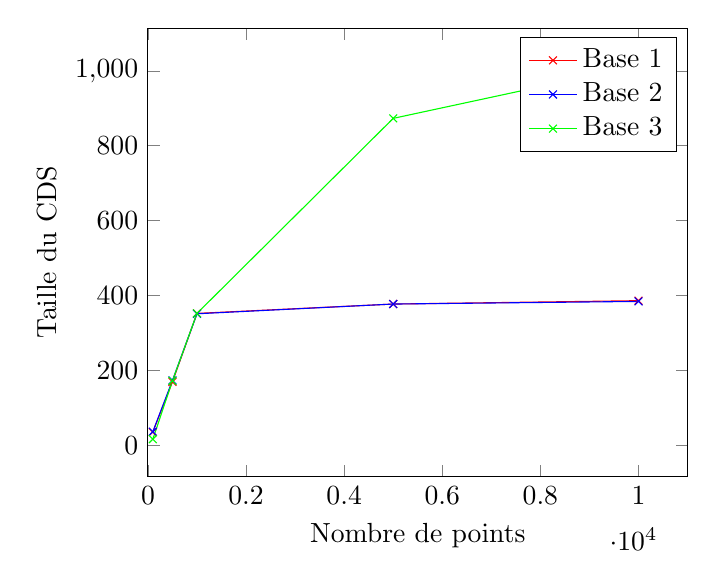
\begin{tikzpicture}
\begin{axis}[%
  xlabel=Nombre de points,
  ylabel=Taille du CDS,
  xmin=0,
]
  \addplot[color=red,mark=x]  coordinates {
	(100, 35)
	(500, 169)
	(1000, 352)
	(5000, 377)
	(10000, 386)
};
  \addlegendentry{Base 1}
  \addplot[color=blue,mark=x]  coordinates {
	(100, 36)
	(500, 173)
	(1000, 351)
	(5000, 377)
	(10000, 384)
};
  \addlegendentry{Base 2}
  \addplot[color=green,mark=x] coordinates {
  	(100, 16)
	(500, 172)
	(1000, 352)
	(5000, 873)
	(10000, 1014)
};
  \addlegendentry{Base 3}
\end{axis}
\end{tikzpicture}
\end{center}
\captionof{figure}{Taille du CDS en fonction du nombre de points avec MIS1}
\end{figure}

BASE 1 ( 1 et 2 correspondent au MIS)
1 - 1 - 100 points - Average size : 35 points - Average time : 0.00129 s - Fails : 0
1 - 2 - 100 points - Average size : 37 points - Average time : 9.1E-4 s - Fails : 0
1 - 1 - 500 points - Average size : 169 points - Average time : 0.0046 s - Fails : 0
1 - 2 - 500 points - Average size : 174 points - Average time : 0.00425 s - Fails : 0
1 - 1 - 1000 points - Average size : 352 points - Average time : 0.01495 s - Fails : 0
1 - 2 - 1000 points - Average size : 364 points - Average time : 0.01403 s - Fails : 0
1 - 1 - 5000 points - Average size : 377 points - Average time : 0.29473 s - Fails : 0
1 - 2 - 5000 points - Average size : 394 points - Average time : 0.25969 s - Fails : 0
1 - 1 - 10000 points - Average size : 386 points - Average time : 1.16013 s - Fails : 0
1 - 2 - 10000 points - Average size : 402 points - Average time : 1.01815 s - Fails : 0

BASE 2 ( 1 et 2 correspondent au MIS)
2 - 1 - 100 points - Average size : 36 points - Average time : 2.0E-4 s - Fails : 0
2 - 2 - 100 points - Average size : 37 points - Average time : 2.4E-4 s - Fails : 0
2 - 1 - 500 points - Average size : 173 points - Average time : 0.00398 s - Fails : 0
2 - 2 - 500 points - Average size : 179 points - Average time : 0.00375 s - Fails : 0
2 - 1 - 1000 points - Average size : 351 points - Average time : 0.0149 s - Fails : 0
2 - 2 - 1000 points - Average size : 365 points - Average time : 0.01398 s - Fails : 0
2 - 1 - 5000 points - Average size : 377 points - Average time : 0.29543 s - Fails : 0
2 - 2 - 5000 points - Average size : 393 points - Average time : 0.26125 s - Fails : 0
2 - 1 - 10000 points - Average size : 384 points - Average time : 1.15217 s - Fails : 0
2 - 2 - 10000 points - Average size : 400 points - Average time : 1.01027 s - Fails : 0

BASE 3 ( 1 et 2 correspondent au MIS)
3 - 1 - 100 points - Average size : 16 points - Average time : 2.9E-4 s - Fails : 0
3 - 2 - 100 points - Average size : 18 points - Average time : 2.4E-4 s - Fails : 0
3 - 1 - 500 points - Average size : 172 points - Average time : 0.0039 s - Fails : 0
3 - 2 - 500 points - Average size : 180 points - Average time : 0.00367 s - Fails : 0
3 - 1 - 1000 points - Average size : 352 points - Average time : 0.01476 s - Fails : 0
3 - 2 - 1000 points - Average size : 365 points - Average time : 0.01395 s - Fails : 0
3 - 1 - 5000 points - Average size : 873 points - Average time : 0.32062 s - Fails : 0
3 - 2 - 5000 points - Average size : 907 points - Average time : 0.28485 s - Fails : 0
3 - 1 - 10000 points - Average size : 1014 points - Average time : 1.20708 s - Fails : 0
3 - 2 - 10000 points - Average size : 1054 points - Average time : 1.0546 s - Fails : 0